\documentclass{beamer}
\usepackage[numbers]{natbib}

% \usepackage{beamerthemesplit} // Activate for custom appearance

\title{W4240/W6240 \\\qquad \\Data Mining/\\Statistical Machine Learning}
\author{Frank Wood}
\date{\today}

\newcommand{\comment}[1]{}


\def\x{\mathbf{x}}
\def\transpose{T}
\def\bmu{\boldsymbol{\mu}}

\def\x{\mathbf{x}}
\def\t{\mathbf{t}}
\def\y{\mathbf{y}}










\newcommand{\ponedec}{\mathcal{P}^\downarrow_1}
\newcommand{\pone}{\mathcal{P}_1}
\newcommand{\rank}[1]{\mathrm{RANK}\left[#1\right]}
\newcommand{\E}[1]{\mathrm{E}\left[#1\right]}
\newcommand{\py}{\mathcal{PY}}
\newcommand{\iid}{iid.}
\newcommand{\drawiid}{\stackrel{\text{iid}}{\sim}}
\newcommand{\vect}[1]{\mathbf{#1}}
\newcommand{\indicator}[1]{\text{I}\left[ #1 \right]}
\newcommand{\pdcoag}{PD(d_1,0)-\text{COAG}}
\newcommand{\todo}{\textbf{*TODO*}}
\newcommand{\igram}{\text{$\infty$-gram}}
\newcommand{\Prob}{\text{P}}

\def\mm{sequence memoizer }
\def\MM{SM }

\def\pibf{{\boldsymbol{\pi}}}
\def\Pibf{{\boldsymbol{\Pi}}}
\def\Thetabf{{\boldsymbol{\Theta}}}
\def\thetabf{{\boldsymbol{\theta}}}

\def\kapbf{\boldsymbol{\kappa}}
\def\taubf{\boldsymbol{\tau}}
\def\thebf{\boldsymbol{\theta}}
\def\rhobf{\boldsymbol{\rho}}
\def\phibf{\boldsymbol{\phi}}
\def\pbf{\mathbf{p}}
\def\qbf{\mathbf{q}}
\def\sbf{\mathbf{s}}
\def\tbf{\mathbf{t}}
\def\ybf{\mathbf{y}}
\def\wbf{\mathbf{w}}
\def\xbf{\mathbf{x}}
\def\zbf{\mathbf{z}}
\def\rbf{\mathbf{r}}
\def\tbf{\mathbf{t}}
\def\kbf{\mathbf{k}}
\def\Xbf{\mathbf{X}}
\def\0bf{\mathbf{0}}
\def\Ibf{\mathbf{I}}
\def\phibf{\mathbf{\phi}}
\def\Phibf{\mathbf{\Phi}}
\def\disteq{{\stackrel{D}{=}}}
\def\EE{{\mathbb{E}}}

\def\phiv{\varphi}
\def\phivbf{\boldsymbol{\varphi}}

\def\Ocal{\mathcal{O}}

\DeclareMathOperator*{\Bet}{Beta}
\DeclareMathOperator{\coag}{COAG}
\DeclareMathOperator{\frag}{FRAG}
\DeclareMathOperator*{\rnk}{RANK}
\DeclareMathOperator*{\gem}{GEM}
\DeclareMathOperator*{\pd}{PD}
\DeclareMathOperator*{\gd}{GDir}
\DeclareMathOperator*{\Dir}{Dir}
\DeclareMathOperator*{\Discrete}{Discrete}
\DeclareMathOperator*{\Mult}{Multinomial}


\begin{document}

\frame[t]{\titlepage}


\section{Introduction}
\subsection{Overview of Topics}

\frame[t] { 
\frametitle{Today: Really Big Picture}
\begin{itemize}
\item The glue that binds the course together : graphical models.
\item A guiding philosophy : Bayesian inference.
\end{itemize}

}


\frame[t] { 
\frametitle{The Glue: Graphical Models}

\begin{itemize}
\item Many probabilistic models can be expressed in the ``language'' of graphical models.  

\end{itemize}

\begin{figure}[htbp]
\begin{center}
\includegraphics{"../prmlfigs-pdf-recolored/Figure8_22a"}\caption{Directed Graphical Model : Chapter 8, Figure 22a, PRML \cite{Bishop2006}}
\label{fig:8_22a}
\end{center}
\end{figure}
\vspace{-.5cm}
\[P(a,b,c,e,f) = P(a)P(f)P(e|a,f)P(b|f)P(c|e)\]
}

\frame[t] { 
\frametitle{Graphical Models Cont.}
\begin{itemize}
\item Correspond (sometimes) to a ``plausible'' generative mechanism.
\item Reveal latent variable choices and help clarify what inferences can be performed
\item Provide datastructure on which inference and estimation algorithms can run
\item Specify conditional indendencies and highlight computational savings

\begin{block}{Course Goal}
Learn how to ``think'' in terms of graphical models.  Be able to write down a generative graphical model for data of interest to you and to know how to do inference in generic graphical models.
\end{block}
\end{itemize}

{\small \em Give ordering Shakespeare example}
}

\frame[t] { 
\frametitle{Example directed graphical model / Bayes net : ALARM, expert diagnostic system}
Goal: Inference in given/known/hand-specified Bayesian network 
\begin{figure}[htbp]
\begin{center}
\includegraphics[width=11cm]{"alarm_network"}\caption{ALARM stands for 'A Logical Alarm Reduction Mechanism'. This is a medical diagnostic system for patient monitoring. It is a nontrivial belief network with 8 diagnoses, 16 findings and 13 intermediate variables. Described in \cite{Beinlich1989}}
\label{fig:1_1}
\end{center}
\end{figure}
}


\frame[t] { 
\frametitle{Inference in discrete directed acyclic graphical models}
Inference procedures known as the \underline{sum-product algorithm} and \underline{belief propagation} are general inference techniques that can easily be adapted to discrete and linear-Gaussian graphical models. \newline

Belief propagation 
\begin{itemize}
\item Computes marginal distributions of any subset of variables in the graphical model conditioned on any other subset of variables (values observed / fixed)
\item Generalizes many, many inference procedures such as Kalman filter, forward-backward, etc.
\item Can be used for parameter estimation in the case where all latent, unknown variables are ``parameters'' and all observations are fixed, known variables.
\end{itemize}
}

\frame[t] {% slide 1
 \frametitle{Bayesian Analysis Recipe}

Bayesian data analysis can be described as a three step process
\begin{enumerate}
\item Set up a full (generative) probability model
\item Condition on the observed data to produce a posterior distribution, the conditional distribution of the unobserved quantities of interest (parameters or functions of the parameters, etc.)
\item Evaluate the goodness of the model
\item Perform inference taking into account the uncertainty about the model parameters encoded in the posterior distribution
\end{enumerate}
}

\frame[t] {% slide 2
 \frametitle{Philosophy}

Gelman, ``Bayesian Data Analysis''
\begin{quotation}\small
A primary motivation for believing Bayesian thinking important is that it facilitates a common-sense interpretation of statistical conclusions.  For instance, a Bayesian (probability) interval for an unknown quantity of interest can be directly regarded as having a high probability of containing the unknown quantity, in contrast to a frequentist (confidence) interval, which may strictly be interpreted only in relation to a sequence of similar inferences that might be made in repeated practice.
\end{quotation}
}

\frame[t] {% slide 3
\frametitle{Theoretical Setup}
Consider a model with parameters $\Theta$ and observations that are independently and identically distributed from some distribution $X_i \sim F(\cdot,\Theta)$ parameterized by $\Theta$.  

Consider a prior distribution on the model parameters $P(\Theta; \Psi)$

\begin{itemize}
\item What does \[P(\Theta |  X_1,\ldots,X_N; \Psi) \propto P( X_1,\ldots,X_N | \Theta; \Psi) P(\Theta; \Psi)\] mean?  
\item What does $P(\Theta; \Psi)$ mean?  What does it represent?
\end{itemize}

In this course we will consider complicated likelihoods and priors (many parameters, often related in non-trivial ways) and the algorithms required to perform inference in such models.

}

\frame[t] {% slide 4
\frametitle{Very Simple Example}

Consider the following example: suppose that you are thinking about purchasing a factory that makes pencils.  Your accountants have determined that you can make a profit (i.e.~you should transact the purchase) if the percentage of defective pencils manufactured by the factory is less than 30\%.  \newline

In your prior experience, you learned that, on average, pencil factories produce defective pencils at a rate of 50\%. \newline

To make your judgement about the efficiency of this factory you test pencils one at a time in sequence as they emerge from the factory to see if they are defective.

}

\frame[t] {% slide 4
\frametitle{Notation}

Let $X_1,\ldots,X_N, X_i \in \{0,1\}$ be a set of defective/not defective observations.  \newline

Let $\Theta$ be the probability of pencil defect.  \newline

Let $P(X_i | \Theta) = \Theta^{X_i}(1-\Theta)^{1-X_i}$ (a Bernoulli random variable)\newline

}

\frame[t] {% slide 5
\frametitle{Typical elements of Bayesian inference}

Two typical Bayesian inference objectives are

\begin{enumerate}
\item The {\em posterior distribution} of the model parameters \[P(\Theta| X_1,\ldots, X_n) \propto P( X_1,\ldots,
X_n|\Theta) P(\Theta) \]  This distribution is used to make statements about the distribution of the unknown or latent quantities in the model.
\item The {\em posterior predictive distribution} \[P(X_n| X_1,\ldots, X_{n-1}) =  \int P( X_n|\Theta) P(\Theta |  X_1,\ldots, X_{n-1}) d\Theta \] This distribution is used to make predictions about the population given the model and a set of observations.
\end{enumerate}

}

\frame[t] {% slide 6
\frametitle{The Prior}

Both the posterior and the posterior predictive distributions require the choice of a prior over model parameters $P(\Theta)$ which itself will usually have some parameters.  If we call those parameters $\Psi$ then you might see the prior written as $P(\Theta; \Psi).$ \newline

The prior encodes your prior belief about the values of the parameters in your model.  The prior has several interpretations and many modeling uses

\begin{itemize}
\item Encoding previously observed, related observations (pseudocounts)
\item Biasing the estimate of model parameters towards more realistic or probable values
\item Regularizing or contributing towards the numerical stability of an estimator
\item Imposing constraints on the values a parameter can take
\end{itemize}
}

\frame[t] {% slide 7
\frametitle{Choice of Prior - Continuing the Example}

In our example the model parameter $\Theta$ can take a value in $\Theta \in [0,1].$  Therefore the prior distribution's support should be $[0,1]$ \newline

One possibility is $P(\Theta) = 1$.  This means that we have no prior information about the value $\Theta$ takes in the real world.  Our prior belief is uniform over all possible values.   \newline

Given our assumptions (that 50\% of manufactured pencils are defective in a typical factory) this seems like a poor choice. \newline

A better choice might be a non-uniform parameterization of the Beta distribution.
}

\frame[t] {% slide 8
\frametitle{Beta Distribution}
The Beta distribution $\Theta \sim \Bet(\alpha,\beta)$ ($\alpha>0, \beta>0, \Theta \in [0,1]$) is a distribution over a single number between 0 and 1.  This number can be interpreted as a probability.  In this case, one can think of $\alpha$ as a pseudo-count related to the number of successes (here a success will be the failure of a pencil) and $\beta$ as a pseudo-count related to the number of failures in a population.   In that sense, the distribution of $\Theta$ encoded by the Beta distribution can produce many different biases. \newline

The formula for the Beta distribution is 
\[ P(\Theta|\alpha, \beta) = \frac{\Gamma(\alpha+\beta)}{\Gamma(\alpha)\Gamma(\beta)}\Theta^{\alpha-1}(1-\Theta)^{\beta-1}\]

{\small Run introduction\_to\_bayes/main.m }


}

\frame[t] {% slide 8
\frametitle{$\Gamma$ function}
In the formula for the Beta distribution 
\[ P(\Theta|\alpha, \beta) = \frac{\Gamma(\alpha+\beta)}{\Gamma(\alpha)\Gamma(\beta)}\Theta^{\alpha-1}(1-\Theta)^{\beta-1}\]

The gamma function (written $\Gamma(x)$) appears. \newline

It can be defined recursively as $\Gamma(x) = (x-1)\Gamma(x-1) = (x-1)!$ with $\Gamma(1) = 1$.\newline

This is just a generalized factorial (to real and complex numbers in addition to integers).  It's value can be computed.  It's derivative can be taken, etc. \newline

Note that, by inspection (and definition of distribution)

\[\int \Theta^{\alpha-1}(1-\Theta)^{\beta-1} d\Theta = \frac{\Gamma(\alpha)\Gamma(\beta)}{\Gamma(\alpha+\beta)}\]


}

\frame[t] {% slide 8
\frametitle{Beta Distribution}
\begin{figure}[htbp]
\begin{center}
 \includegraphics[width=.5\textwidth]{beta_p1_p1.pdf} % requires the graphicx package
\caption{Beta(.1,.1)}
\end{center}
\end{figure}


}


\frame[t] {% slide 8
\frametitle{Beta Distribution}
\begin{figure}[htbp]
\begin{center}
 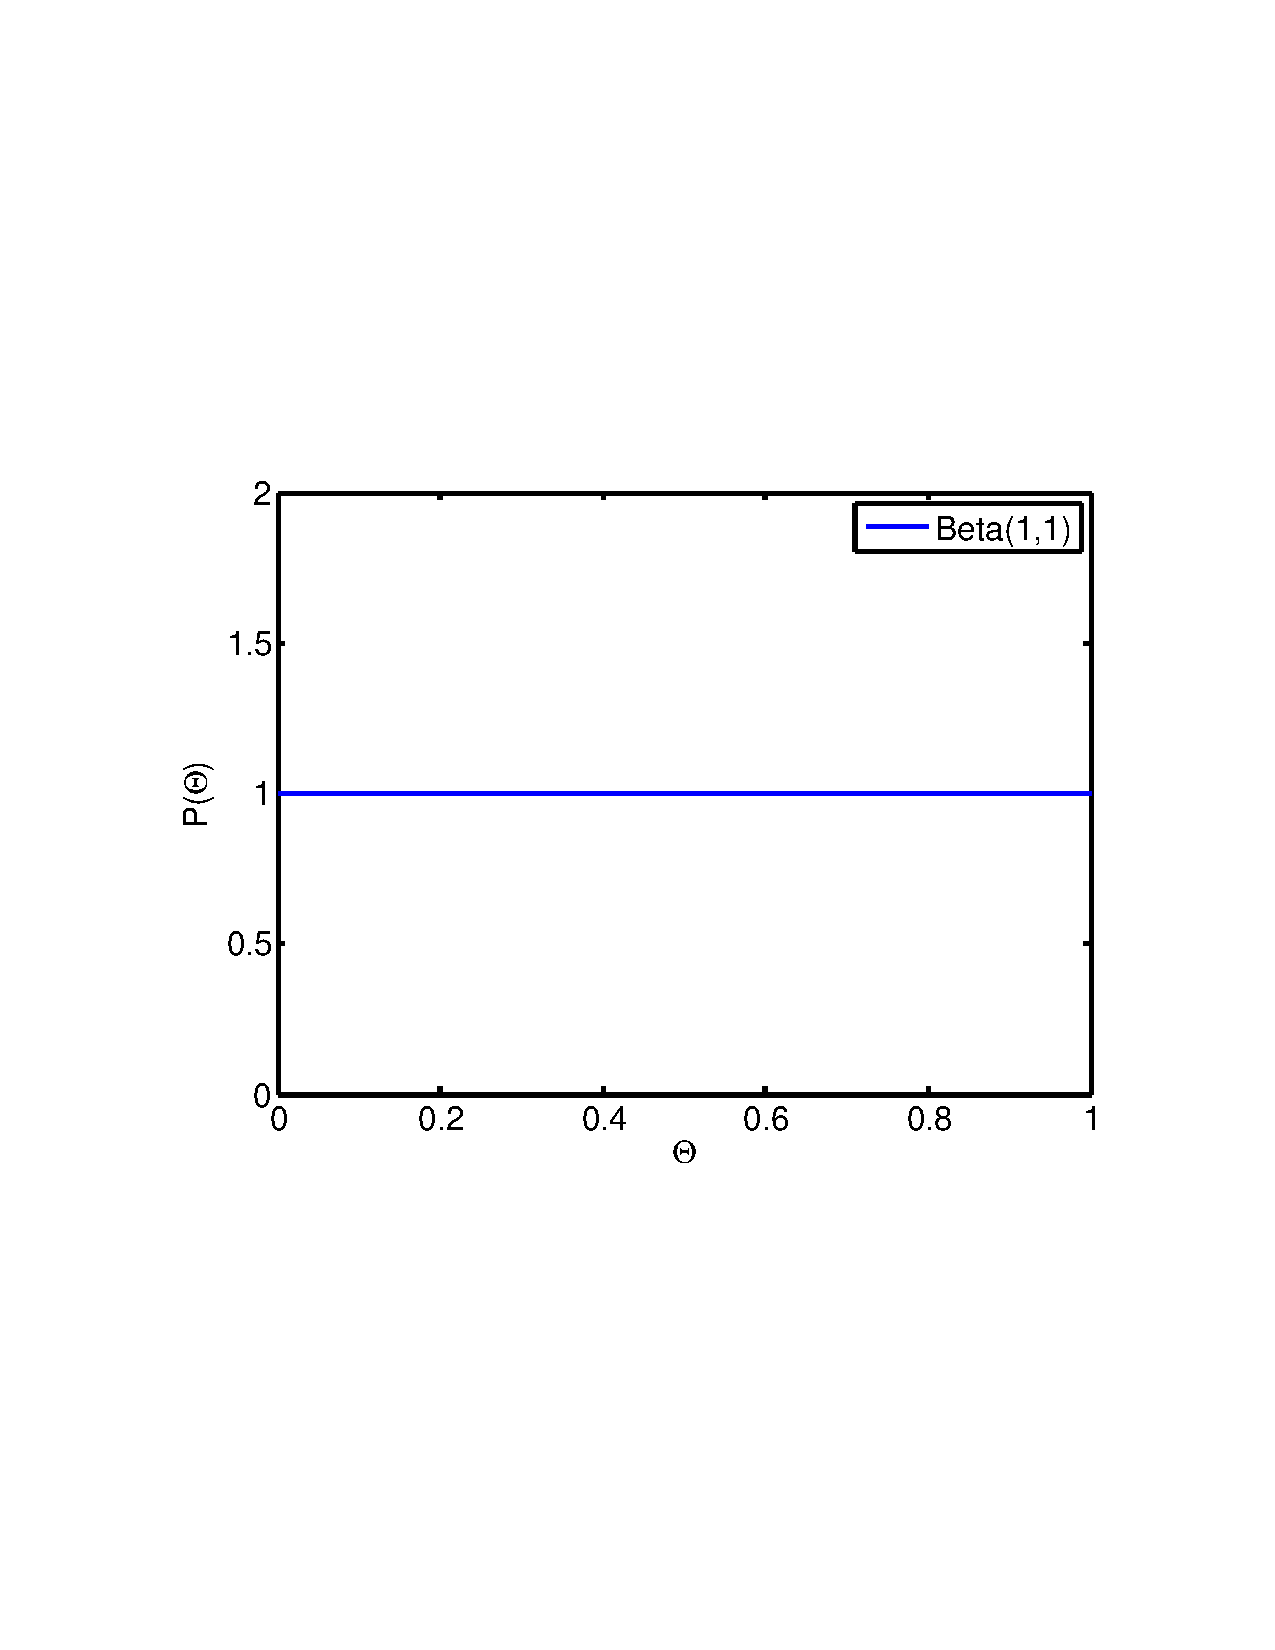
\includegraphics[width=.5\textwidth]{beta_1_1.pdf} % requires the graphicx package
\caption{Beta(1,1)}
\end{center}
\end{figure}


}

\frame[t] {% slide 8
\frametitle{Beta Distribution}
\begin{figure}[htbp]
\begin{center}
 \includegraphics[width=.5\textwidth]{beta_5_5.pdf} % requires the graphicx package
\caption{Beta(5,5)}
\end{center}
\end{figure}


}

\frame[t] {% slide 8
\frametitle{Beta Distribution}
\begin{figure}[htbp]
\begin{center}
 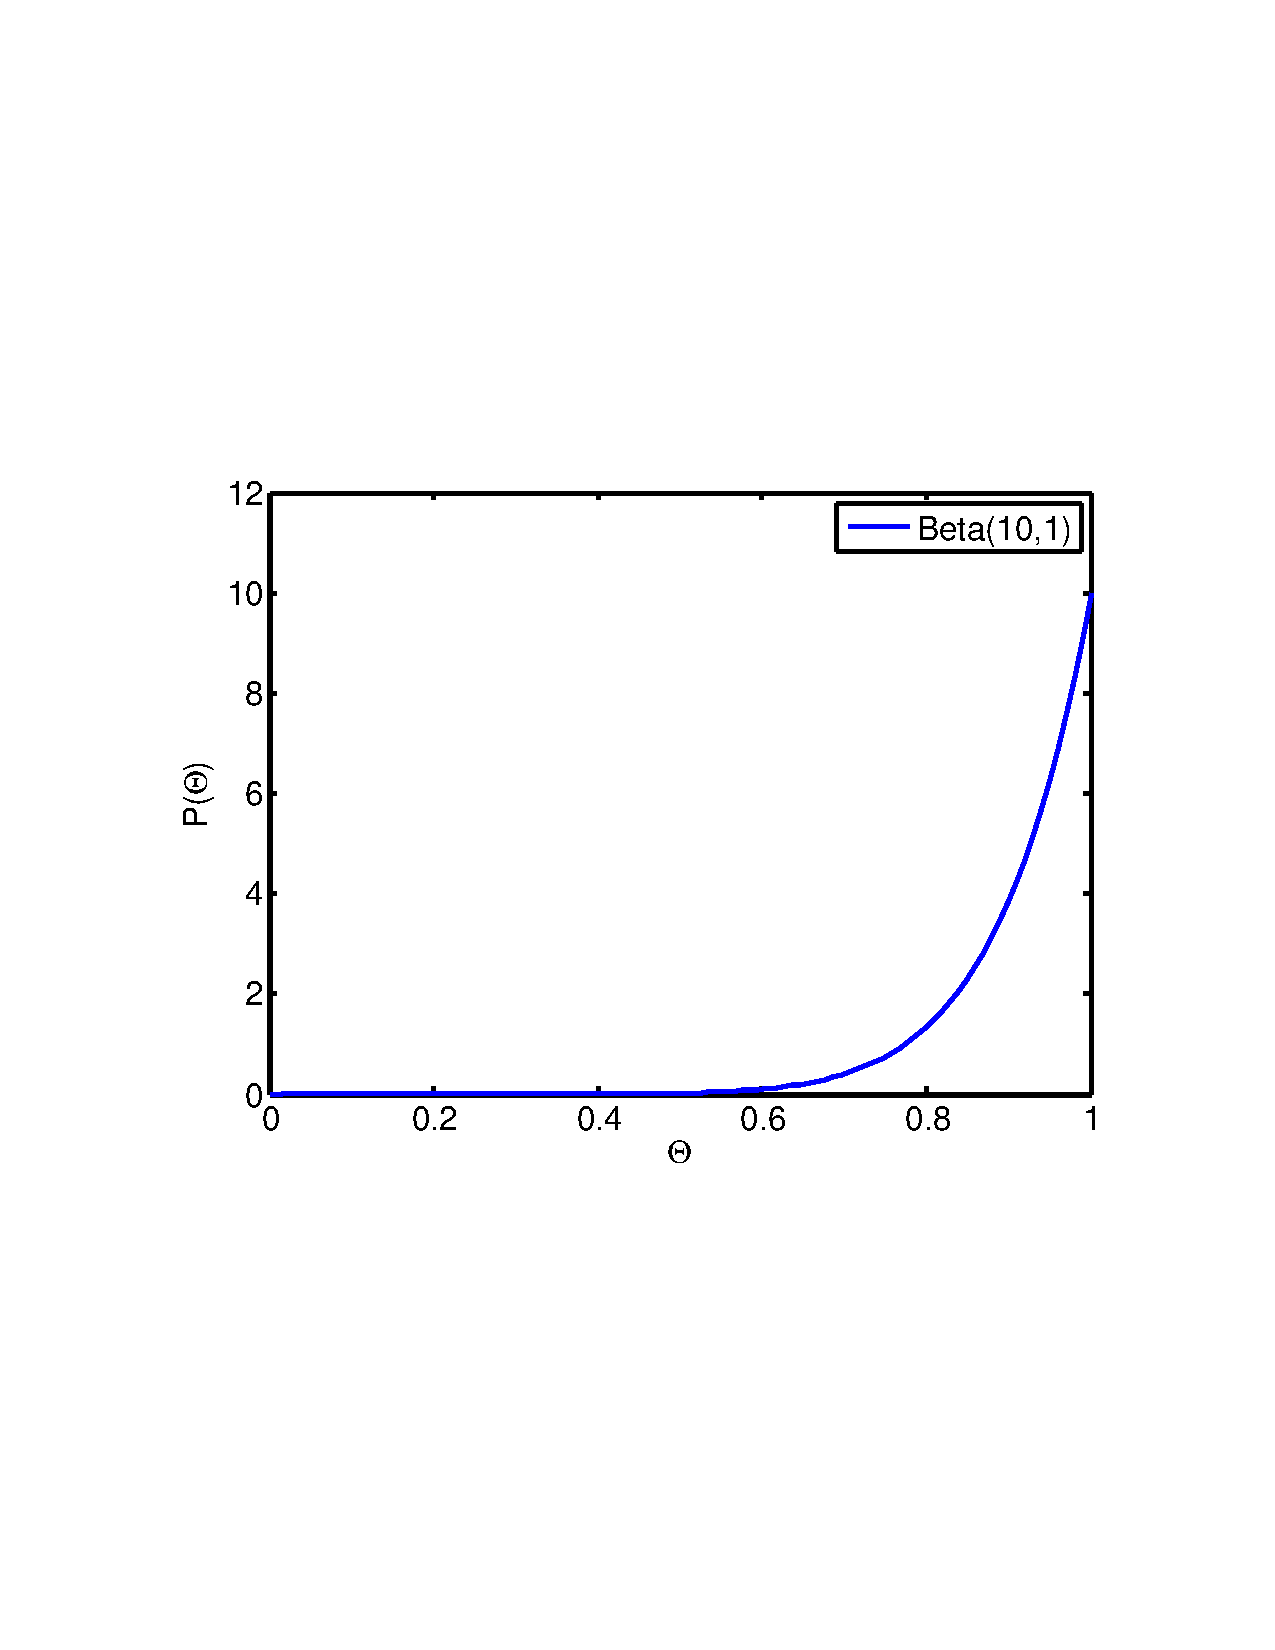
\includegraphics[width=.5\textwidth]{beta_10_1.pdf} % requires the graphicx package
\caption{Beta(10,1)}
\end{center}
\end{figure}


}

\frame[t] {% slide 8
\frametitle{Generative Model}
With the introduction of this prior we now have a full generative model of our data (given $\alpha$ and $\beta$, the model's hyperparameters).  

Consider the following procedure for generating pencil failure data:

\begin{itemize}
\item Sample a failure rate parameter $\Theta$ for the ``factory'' from a $\Bet(\alpha, \beta)$ distribution.  This yields the failure rate for the factory.
\item Given the failure rate $\Theta$, sample $N$ defect/no-defect observations from a Bernoulli distribution with parameter $\Theta.$
\end{itemize}

Bayesian inference involves ``turning around'' this generative model, i.e.~uncovering a distribution over the parameter $\Theta$ given both the observations and the prior. \newline

This class will be about the general purpose computations necessary to do this.

}


\frame[t] {% slide 8
\frametitle{Inferring the Posterior Distribution}

Remember that the {\em posterior distribution} of the model parameters is given by Bayes rule, here \[P(\Theta| X_1,\ldots, X_n) \propto P( X_1,\ldots,
X_n|\Theta) P(\Theta) \] 
Let's consider what the posterior looks like after observing a single observation (in our example). \newline

Our likelihood is given by \[ P( X_1|\Theta) = \Theta^{X_1}(1-\Theta)^{1-X_1}\]

Our prior, the Beta distribution, is given by 
\[ P(\Theta) = \frac{\Gamma(\alpha+\beta)}{\Gamma(\alpha)\Gamma(\beta)}\Theta^{\alpha-1}(1-\Theta)^{\beta-1}\]
}

\frame[t] {% slide 8
\frametitle{Analytic Posterior Update - No Computation}

Since we know that \[P(\Theta| X_1) \propto P( X_1|\Theta) P(\Theta) \] we can write 

 \[P(\Theta| X_1) \propto  \Theta^{X_1}(1-\Theta)^{1-X_1} \frac{\Gamma(\alpha+\beta)}{\Gamma(\alpha)\Gamma(\beta)}\Theta^{\alpha-1}(1-\Theta)^{\beta-1}\]
 but since we are interested in a function (distribution) of $\Theta$ and we are working with a proportionality, we can throw away terms that do not involve $\Theta$ yielding
 \[P(\Theta| X_1) \propto   \Theta^{\alpha+X_1-1}(1-\Theta)^{1-X_1+\beta-1}\]
 Because of {\em conjugacy} we have an analytic form for the posterior distribution of the model parameters of the data.  The class is about similar computation in more difficult models.   \newline
 Note that this is an incremental procedure.
}

\frame[t] {% slide 8
\frametitle{Bayesian Computation, Implicit Integration}
From the previous slide we have
 \[P(\Theta| X_1) \propto   \Theta^{\alpha+X_1-1}(1-\Theta)^{1-X_1+\beta-1}\]
To make this proportionality an equality (i.e.~to construct a properly normalized distribution) we have to integrate this expression w.r.t.~$\Theta$, i.e.
 \[P(\Theta| X_1) =  \frac{\Theta^{\alpha+X_1-1}(1-\Theta)^{1-X_1+\beta-1}}{\int \Theta^{\alpha+X_1-1}(1-\Theta)^{1-X_1+\beta-1} d\Theta}\]
 But in this and other special cases like it (when the likelihood and the prior form a conjugate pair) this integral can be solved by recognizing the form of the distribution, i.e.~note that this expression looks exactly like a Beta distribution but with updated parameters, $\alpha_1 = \alpha+X_1, \beta_1 = \beta + 1 - X_1$
 }
 
\frame[t] {% slide 8
\frametitle{Posterior and Repeated Observations}

This yields the following pleasant result

\[\Theta | X_1, \alpha, \beta \sim \Bet(\alpha+X_1, \beta + 1 - X_1)\]

This means that the posterior distribution of $\Theta$ given an observation is in the same parametric family as the prior.  This is characteristic of conjugate  likelihood/prior pairs.  \newline

Note the following decomposition

\[ P(\Theta | X_1, X_2, \alpha, \beta) \propto P(X_2| \Theta, X_1) P(\Theta | X_1, \alpha, \beta)  \]

This means that the preceding posterior update procedure can be repeated.  This is because $P(\Theta | X_1, \alpha, \beta)$ is in the same family (Beta) as the original prior.  The posterior distribution of $\Theta$ given two observations will still be Beta distributed, now just with further updated parameters.
 }
 
 \frame[t] {% slide 8
\frametitle{Incremental Posterior Inference}

Starting with 

\[\Theta | X_1, \alpha, \beta \sim \Bet(\alpha+X_1, \beta + 1 - X_1)\]

and adding $X_2$ we can almost immediately identify 

\[\Theta | X_1, X_2, \alpha, \beta \sim \Bet(\alpha+X_1+X_2, \beta + 1 - X_1 +1 -X_2)\]

which simplifies to 

\[\Theta | X_1, X_2, \alpha, \beta \sim \Bet(\alpha+X_1+X_2, \beta + 2 - X_1 -X_2)\]

and generalizes to 

\[\Theta | X_1, \ldots, X_N, \alpha, \beta \sim \Bet(\alpha+\sum X_i, \beta + N -\sum X_i)\]
 }
 
\frame[t] {% slide 8
\frametitle{Interpretation, Notes, and Caveats}
\begin{itemize}
\item The posterior update computation performed here is unusually simple in that it is analytically tractable.  The integration necessary to normalize the posterior distribution is more often not analytically tractable than it is analytically tractable.  When it is not analytically tractable other methods must be utilized to get an estimate of the posterior distribution -- numerical integration and Markov chain Monte Carlo (MCMC) amongst them.
\item The posterior distribution can be interpreted as the distribution of the model parameters given both the structural assumptions made in the model selection step and the selected prior parameterization.  Asking questions like, ``What is the probability that the factory has a defect rate of less than 10\%?'' can be answered through operations on the posterior distribution.
\end{itemize}

 }
 
 \frame[t] {% slide 8
\frametitle{More Interpretation, Notes, and Caveats}
The posterior can be seen in multiple ways
\begin{eqnarray*}
 P(\Theta| X_{1:N}) &\propto& P( X_1,\ldots,
X_N|\Theta) P(\Theta) \\
&\propto& P( X_N | X_{1:N-1},\Theta) P(X_{N-1} | X_{1:N-2},\Theta) \cdots P(X_{1}|\Theta) P(\Theta) \\
&\propto& P( X_N | \Theta) P(X_{N-1}|\Theta) \cdots P(X_{1}|\Theta) P(\Theta) 
\end{eqnarray*}
(when $X$'s are iid given $\Theta$ or exchangeable) and
\begin{eqnarray*}
 P(\Theta| X_1,\ldots, X_N) &\propto& P( X_N,\Theta | X_1\ldots, X_{N-1})\\
&\propto&  P( X_N|\Theta) P(\Theta | X_1\ldots, X_{N-1})\\
\end{eqnarray*}

The first decomposition highlights the fact that the posterior distribution is influenced by each observation. \newline

The second recursive decomposition highlights the fact that the posterior distribution can be interpreted as the full characterization of the uncertainty about the hidden parameters after having  accounted for all observations to some point.
 }
 
  \frame[t] {% slide 8
\frametitle{Posterior Predictive Inference}
Now that we know how to update our prior beliefs about the state of latent variables in our model we can consider posterior predictive inference.  \newline

Posterior predictive inference performs a weighted average prediction of future values over all possible settings of the model parameters.  The prediction is weighted by the posterior probability of the model parameter setting, i.e.

\[P(X_{N+1} | X_{1:N} ) = \int P(X_{N+1} | \Theta) P(\Theta | X_{1:N})d\Theta\]

Note that this is just the likelihood convolved against the posterior distribution having accounted for $N$ observations.
 }
 
   \frame[t] {% slide 8
\frametitle{More Implicit Integration}
If we return to our example we have the updated posterior distribution
\[\Theta | X_1, \ldots, X_N, \alpha, \beta \sim \Bet(\alpha+\sum_{i=1}^N X_i, \beta + N -\sum_{i=1}^N X_i)\]
and the likelihood of the $(N+1)^{th}$ observation
\[ P( X_{N+1}|\Theta) = \Theta^{X_{N+1}}(1-\Theta)^{1-X_{N+1}}\]
Note that the following integral is similar in many ways to the posterior update
\[P(X_{N+1} | X_{1:N} ) = \int P(X_{N+1} | \Theta) P(\Theta | X_{1:N})d\Theta\]
which means that in this case (and in all conjugate pairs) this is easy to do.
 }
 
    \frame[t] {% slide 8
\frametitle{More Implicit Integration}

\begin{eqnarray*}
P(X_{N+1} | X_{1:N} )& =& \int\Theta^{X_{N+1}}(1-\Theta)^{1-X_{N+1}} \\
&\times& \frac{\Gamma(\alpha+\beta + N)}{\Gamma(\alpha+\sum_{i=1}^N X_i)\Gamma(\beta + N -\sum_{i=1}^N X_i)} \\
&\times& \Theta^{\alpha+\sum_{i=1}^N X_i-1}(1-\Theta)^{\beta + N -\sum_{i=1}^N X_i)-1}d\Theta
\end{eqnarray*}
\begin{eqnarray*}
& =&  \frac{\Gamma(\alpha+\beta + N)}{\Gamma(\alpha+\sum_{i=1}^N X_i)\Gamma(\beta + N -\sum_{i=1}^N X_i)} \\
&\times&  \frac{\Gamma(\alpha+\sum_{i=1}^N X_i + X_{N+1})\Gamma(\beta + N+1 -\sum_{i=1}^N X_i - X_{N+1})}{\Gamma(\alpha+\beta + N+1)} \\
\end{eqnarray*}
 }
 
     \frame[t] {% slide 8
\frametitle{Interpretation}
\begin{eqnarray*}
\lefteqn{P(X_{N+1} | X_{1:N} )}\\
 &=&  \frac{\Gamma(\alpha+\beta + N)}{\Gamma(\alpha+\sum_{i=1}^N X_i)\Gamma(\beta + N -\sum_{i=1}^N X_i)} \\
&\times&  \frac{\Gamma(\alpha+\sum_{i=1}^N X_i + X_{N+1})\Gamma(\beta + N+1 -\sum_{i=1}^N X_i - X_{N+1})}{\Gamma(\alpha+\beta + N+1)} \\
\end{eqnarray*}
 Is a ratio of Beta normalizing constants. \newline
 
 This a distribution over $[0,1]$ which averages over all possible models in the family under consideration (again, weighted by their posterior probability). 

 }
 
      \frame[t] {% slide 8
\frametitle{Caveats again}
In posterior predictive inference many of the same caveats apply.  

\begin{itemize}
\item Inference can be computationally demanding if conjugacy isn't exploited.
\item Inference results are only as good as the model and the chosen prior.  
\end{itemize}
But Bayesian inference has some pretty big advantages
\begin{itemize}
\item Assumptions are explicit and easy to characterize.
\item It is easy to plug and play Bayesian models.
\end{itemize}

 }
 
 
\frame[t] {% slide 8
\frametitle{Beta Distribution}
\begin{figure}[htbp]
\begin{center}
 \includegraphics[width=.5\textwidth]{posterior.pdf} % requires the graphicx package
\caption{Posterior after 1000 observations.}
\end{center}
\end{figure}


}


\frame[t] {% slide 8
\frametitle{Beta Distribution}
\begin{figure}[htbp]
\begin{center}
 \includegraphics[width=.5\textwidth]{posterior_predictive.pdf} % requires the graphicx package
\caption{Posterior predictive after 1000 observations.}
\end{center}
\end{figure}


}


\frame[t] { 
\frametitle{More complicated models}
It is possible to extend this generative framework to model more complicated phenomena.  The basics stay the same, computation just gets harder. \newline
Canonical examples include
\begin{itemize}
\item Classification of handwritten digits
\item Trajectory inference
\item Clustering
\end{itemize}
}


\frame[t] { 
\frametitle{Digit classification cast as probabilistic modeling challenge}
Goal
\begin{itemize}
\item Build a machine that can identify handwritten digits automatically
\end{itemize}
Approaches
\begin{itemize}
\item Hand craft a set of rules that separate each digit from the next
\item Set of rules invariably grows large and unwieldy and requires many ``exceptions''
\item ``Learn'' a set of models for each digit automatically from labeled training data, i.e.~{\em mine} a large collection of handwritten digits and produce a model of each
\item Use model to do classification
\end{itemize}
Formalism
\begin{itemize}
\item Each digit is 28x28 pixel image
\item Vectorized into a 784 entry vector $\x$ 
\end{itemize}
}

\frame[t] { 
\frametitle{Handwritten Digit Recognition Training Data}
\begin{figure}[htbp]
\begin{center}
\includegraphics{"../prmlfigs-pdf-recolored/Figure1_1"}\caption{Hand written digits from the USPS}
\label{fig:1_1}
\end{center}
\end{figure}
}


\frame[t] { 
\frametitle{Machine learning approach to digit recognition}
Recipe
\begin{itemize}
\item Obtain a of $N$ digits $\{\x_1, \ldots, \x_N\}$ called the {\em training set}.
\item Label (by hand) the training set to produce a label or ``target'' $\t$ for each digit image $\x$
\item Learn a function $\y(\x)$ which takes an image $\x$ as input and returns an output in the same ``format'' as the target vector.
\end{itemize}
Terminology
\begin{itemize}
\item The process of determining the precise shape of the function $\y$ is known as the ``training'' or ``learning'' phase.
\item After training, the model (function $\y$) can be used to figure out what digit unseen images might be of.  The set comprised of such data is called the ``test set''
\end{itemize}

}

\frame[t] { 
\frametitle{Tools for the handwriting recognition job}
Supervised Regression/Classification Models
\begin{itemize}
\item Logistic regression
\item Neural networks
\item Support vector machines
\item Naive Bayes classifiers
\end{itemize}
Unsupervised Clustering
\begin{itemize}
\item Gaussian mixture model
\end{itemize}

Model Parameter Estimation
\begin{itemize}
\item Maximum likelihood / Expectation Maximization
\item Variational inference
\item Sampling
\item Sequential Monte Carlo
\begin{itemize}
\item... for all, batch or online
\end{itemize}
\end{itemize}

}


\frame[t] { 
\frametitle{Example Application: Trajectory Inference From Noisy Data}
Goal
\begin{itemize}
\item Build a machine that can uncover and compute the true trajectory of an indirectly and noisily observed moving target
\end{itemize}
Approaches
\begin{itemize}
\item Hand craft a set of rules that govern the possible movements of said target
\item Set of rules invariably grows large and unwieldy and requires many ``exceptions''
\item ``Learn'' a model of the kind of movements such a target can make and perform inference in said model
\end{itemize}
Formalism
\begin{itemize}
\item Example observed trajectories $\{\xbf_{n}\}_{n=1}^N$
\item Unobserved latent trajectories $\{\zbf_{n}\}_{n=1}^N$ 
\end{itemize}
}

\frame[t] { 
\frametitle{Latent trajectory Inference}
\begin{figure}[htbp]
\begin{center}
\includegraphics[width=8cm]{"bomb_tracking"}\caption{Schematic of trajectory inference problem}
\label{fig:1_1}
\end{center}
\end{figure}
}

\frame[t] { 
\frametitle{Tools for Latent Trajectory Inference}
Known/hand-crafted model, inference only
\begin{itemize}
\item Belief propagation
\item Kalman filter
\item Particle filter
\item Switching variants thereof
\item Hidden Markov Models
\end{itemize}
Learning too / Model Parameter Estimation
\begin{itemize}
\item Maximum likelihood / Expectation Maximization
\item Variational inference
\item Sampling
\item Sequential Monte Carlo
\begin{itemize}
\item... for all, batch or online
\end{itemize}
\end{itemize}

Trajectory need not be ``physical,'' could be an economic indicator, completely abstract, etc.
}

\frame[t] { 
\frametitle{Cool Trajectory Inference Application : Neural Decoding}
\begin{figure}[htbp]
\begin{center}
\includegraphics[trim = 20mm 20mm 20mm 50mm, clip, width=10cm]{"neural_decoding"}\caption{Actual and predicted hand positions (predicted from neural firing rates alone using a Kalman filter) \cite{Wu2002}}
\label{fig:1_1}
\end{center}
\end{figure}
}


\frame[t] { 
\frametitle{Another Application: Unsupervised Clustering}
Forensic analysis of printed documents, infer printer used to print document from visual features.
\begin{figure}[htbp]
\begin{center}
\includegraphics[width=6cm]{"printer_clustering"}\caption{PCA projection of printer features \cite{Ali2004}}
\label{fig:1_1}
\end{center}
\end{figure}

}

\frame[t] { 
\frametitle{Another Unsupervised Clustering Application}
Automatic discovery of number of neurons and assignment of waveforms to neurons.  Essential to electrophysiological study of the brain.
\begin{figure}[htbp]
\begin{center}
\includegraphics[width=6cm]{"sorted_waveforms"}\caption{Automatically sorted action potential PCA projections \cite{Wood2008b}}
\label{fig:1_1}
\end{center}
\end{figure}

}

\frame[t] { 
\frametitle{A Big Unsupervised Clustering Application}
Multinomial mixture model automatic document clustering for information retrieval.

\begin{eqnarray*}
z_n | \pibf &\sim& \Discrete(\pibf) \\
\xbf_n | z_n = k, \Thetabf &\sim& \Mult(\thetabf_{z_n})
\end{eqnarray*}

where $\xbf_n$ is a bag of words or feature representation of a document, $z_n$ is a per document class indicator variable, $ \Thetabf = \{\thetabf_k\}_{k=1}^K$ is a collection of probability vectors over types (or features) (per cluster $k$), and $\pibf = [\pi_1, \ldots, \pi_K], \sum_k \pi_k = 1$ is the class prior.
\newline

Such a model can be used to cluster similar documents together for information retrieval (Google, Bing, etc.) purposes.
}

\frame[t] { 
\frametitle{Tools for Unsupervised Clustering}
Known/hand-crafted model, inference only
\begin{itemize}
\item K-means
\item Gaussian mixture models
\item Multinomial mixture models
\end{itemize}
Learning too / Model Parameter Estimation
\begin{itemize}
\item Maximum likelihood / Expectation Maximization
\item Variational inference
\item Sampling
\item Sequential Monte Carlo
\begin{itemize}
\item... for all, batch or online
\end{itemize}
\end{itemize}
}

\frame[t] { 
\frametitle{Tools for All}
\begin{itemize}
\item Maximum likelihood / Expectation Maximization
\item Variational inference
\item Sampling
\item Sequential Monte Carlo
\begin{itemize}
\item... for all, batch or online
\end{itemize}
\end{itemize}
}



	\bibliographystyle{plainnat}
	\begin{frame}[t,allowframebreaks]{Bibliograpy}

\bibliography{../../../../../papers/uber.bib}
\end{frame}



\end{document}
